\documentclass{article}

\usepackage[utf8]{inputenc}
\usepackage[brazil]{babel}

\title{Homework 1: Perceptron Simples}
\author{Rúbia Reis Guerra \\ 2013031143}

\usepackage{Sweave}
\begin{document}
\Sconcordance{concordance:perceptron.tex:perceptron.rnw:%
1 8 1 1 0 11 1 1 2 1 0 1 1 1 4 2 0 2 1 1 4 2 0 1 3 1 0 1 1 1 5 3 0 1 1 %
1 2 5 0 1 2 1 1 1 3 2 0 1 1 1 2 1 0 2 1 4 0 1 2 3 1 1 4 3 0 2 1 1 3 1 0 %
1 11 10 0 1 4 2 0 1 1 1 2 1 0 2 1 4 0 1 2 3 1 1 5 4 0 1 3 1 0 1 1 4 0 1 %
2 2 1}

\maketitle

\section{Perceptron Simples}
No contexto de redes neurais, um perceptron é um neurônio artificial que utiliza a função degrau de Heaviside como função de ativição. A atividade proposta teve como objetivo o estudo e a implementação de um perceptron de camada única, que corresponde à rede neural \textit{feedforward} mais simples existente. 

%##################################

\subsection{Implementação}
Inicialmente, geram-se duas distribuições de duas variáveis ($x_{1}$,$x_{2}$), caracterizadas por $\mathcal{N}(2,2,\sigma^2)$ e $\mathcal{N}(4,4,\sigma^2)$.

\begin{Schunk}
\begin{Sinput}
> rm(list=ls())
> library('plot3D')
> ####################################
> # Parâmetros #
> N <- 100
> minseq <- 0
> maxseq <- 6
> ####################################
> # Vetor de pesos #
> w <- c(1,1,-6)
> # Gerando dados amostrados das distribuições m1=(2,2)', m2=(4,4)' #
> xc1 <- matrix(rnorm(N*2),ncol=2)*0.5+c(2,2)
> xc2 <- matrix(rnorm(N*2),ncol=2)*0.5+c(4,4)
> ####################################
> # Plot dos dados #
> plot(xc1[,1], xc1[,2], col='red', type='p', xlim=c(minseq,maxseq), 
+      ylim=c(minseq,maxseq), xlab='x_1', ylab='x_2')
> par(new=T)
> plot(xc2[,1], xc2[,2], col='blue', type='p', xlim=c(minseq,maxseq), 
+      ylim=c(minseq,maxseq), xlab='', ylab='')
\end{Sinput}
\end{Schunk}
\includegraphics{perceptron-001}

Deseja-se mostrar que a saída do perceptron em $R^2$ coincide com o separador linear de equação $x_{2} = - x_{1} + 6$, dado o vetor de pesos $w = (1,1,-6)$, igual aos parâmetros da reta.
\begin{Schunk}
\begin{Sinput}
> plot(xc1[,1], xc1[,2], col='red', type='p', xlim=c(minseq,maxseq), 
+      ylim=c(minseq,maxseq),xlab='x_1',ylab='x_2')
> par(new=T)
> plot(xc2[,1], xc2[,2], col='blue', type='p', xlim=c(minseq,maxseq), 
+      ylim=c(minseq,maxseq), xlab='',ylab='')
> par(new=T)
> curve(-x+6,0,6, col='orange', xlab='', ylab='')
\end{Sinput}
\end{Schunk}
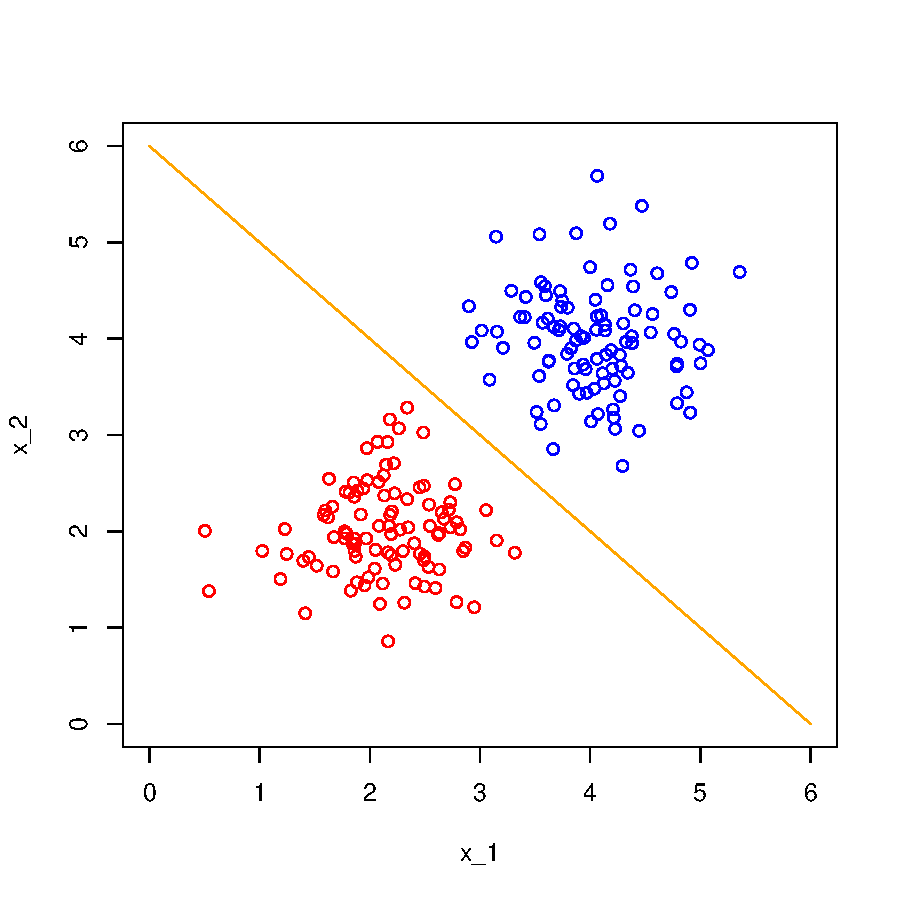
\includegraphics{perceptron-002}

\subsection{Perceptron}
A seguir, implmenta-se a função perceptron percorrendo o espaço $R^2$. Observa-se que a superfície de contorno obtida corresponde à esperada.

\begin{Schunk}
\begin{Sinput}
> ####################################
> # Perceptron  #
> seqi <- seq(minseq,maxseq,0.1)
> seqj <- seq(minseq,maxseq,0.1)
> M <- matrix(1,nrow =length(seqi),ncol=length(seqj))
> # Percorrer o espaço e gerar a saída #
> ci <- 0
> for (i in seqi)
+ {
+   ci <- ci+1
+   cj <- 0
+   for (j in seqj)
+   {
+     cj <- cj + 1
+     xt <- c(i,j,1)
+     M[ci,cj] <- 1*((t(w) %*% xt) >= 0)
+   }
+ }
> # Resposta em R2 #
> plot(xc1[,1], xc1[,2], col='red', type='p', xlim=c(minseq,maxseq), 
+      ylim=c(minseq,maxseq),xlab='x_1',ylab='x_2')
> par(new=T)
> plot(xc2[,1], xc2[,2], col='blue', type='p', xlim=c(minseq,maxseq), 
+      ylim=c(minseq,maxseq),xlab='',ylab='')
> par(new=T)
> contour(seqi,seqj,M)
\end{Sinput}
\end{Schunk}
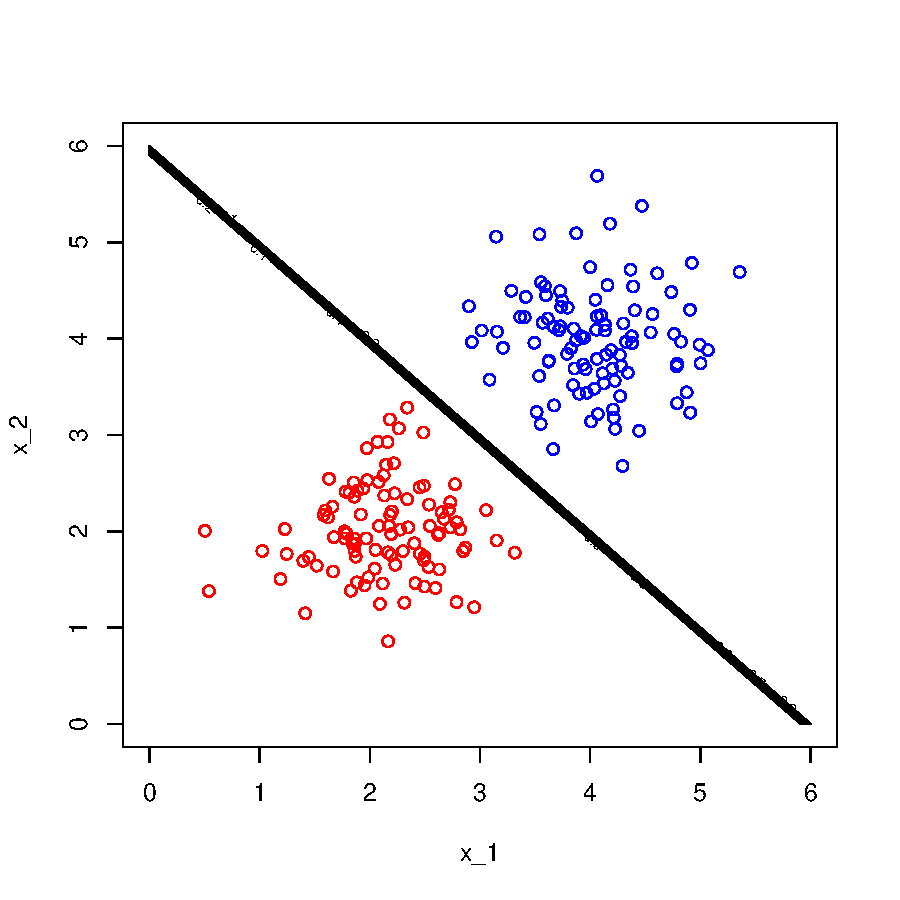
\includegraphics{perceptron-003}


\subsection{Superfície}
Plot da superfície de separação gerada pela função perceptron:
\begin{Schunk}
\begin{Sinput}
> ####################################
> # Superfície de separação #
> ribbon3D(seqi,seqj,M, xlim=c(minseq,maxseq), ylim=c(minseq,maxseq), 
+          zlim=c(0,1), contour=T, add=F, axes=T, ticktype="detailed")
> # Dados #
> scatter3D(xc1[,1],xc1[,2], matrix(0,nrow=dim(xc1)[1]),add=T,col='red')
> scatter3D(xc2[,1],xc2[,2], matrix(0,nrow=dim(xc2)[1]),add=T,col='blue')
\end{Sinput}
\end{Schunk}
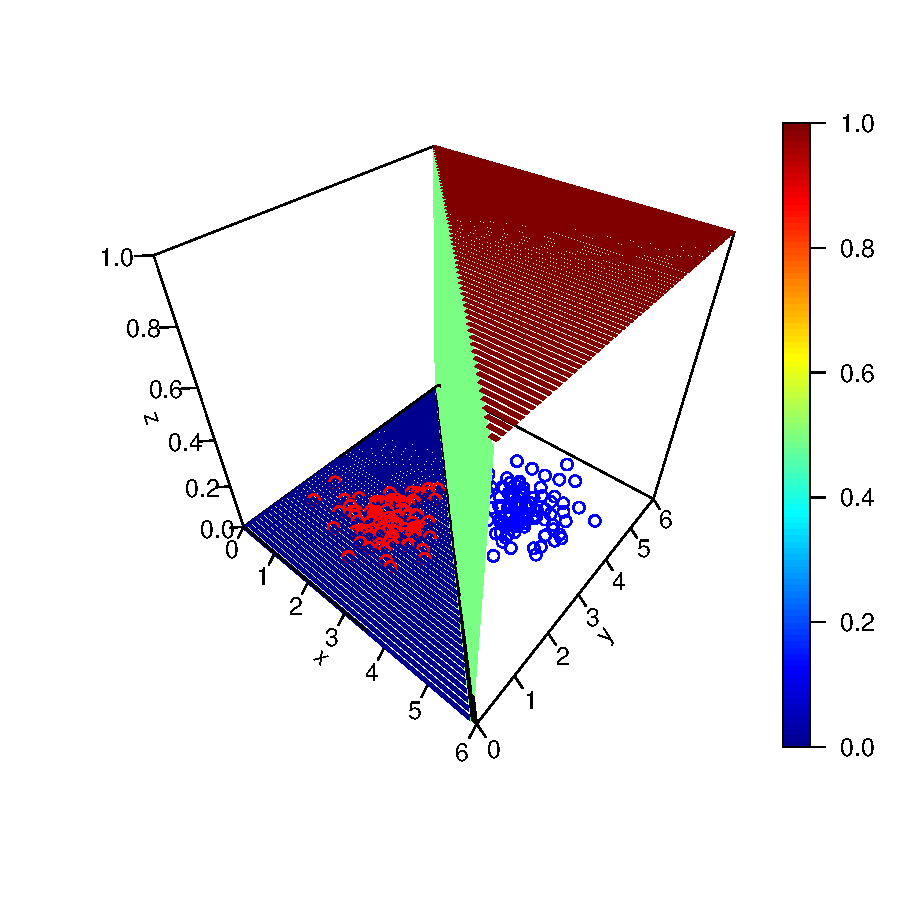
\includegraphics{perceptron-004}


\end{document}
